  
\documentclass{beamer}
\usepackage{listings}
\lstset{
%language=C,
frame=single, 
breaklines=true,
columns=fullflexible
}
\usepackage{blkarray}
\usepackage{subcaption}
\usepackage{url}
\usepackage{tikz}
\usepackage{tkz-euclide} % loads  TikZ and tkz-base
%\usetkzobj{all}
\usetikzlibrary{calc,math}
\usepackage{float}
\newcommand\norm[1]{\left\lVert#1\right\rVert}
\renewcommand{\vec}[1]{\mathbf{#1}}
\usepackage[export]{adjustbox}
\usepackage[utf8]{inputenc}
\usepackage{amsmath}
\usepackage{tikz}
\usetikzlibrary{automata, positioning}
\usetheme{Boadilla}
\providecommand{\pr}[1]{\ensuremath{\Pr\left(#1\right)}}
\providecommand{\mbf}{\mathbf}
\providecommand{\pr}[1]{\ensuremath{\Pr\left(#1\right)}}
\providecommand{\qfunc}[1]{\ensuremath{Q\left(#1\right)}}
\providecommand{\fn}[1]{\ensuremath{f\left(#1\right)}}
\providecommand{\e}[1]{\ensuremath{E\left(#1\right)}}
\providecommand{\sbrak}[1]{\ensuremath{{}\left[#1\right]}}
\providecommand{\lsbrak}[1]{\ensuremath{{}\left[#1\right.}}
\providecommand{\rsbrak}[1]{\ensuremath{{}\left.#1\right]}}
\providecommand{\brak}[1]{\ensuremath{\left(#1\right)}}
\providecommand{\lbrak}[1]{\ensuremath{\left(#1\right.}}
\providecommand{\rbrak}[1]{\ensuremath{\left.#1\right)}}
\providecommand{\cbrak}[1]{\ensuremath{\left\{#1\right\}}}
\providecommand{\lcbrak}[1]{\ensuremath{\left\{#1\right.}}
\providecommand{\rcbrak}[1]{\ensuremath{\left.#1\right\}}}
\theoremstyle{remark}
\newtheorem{rem}{Remark}
\newcommand{\sgn}{\mathop{\mathrm{sgn}}}
\newcommand{\comb}[2]{{}^{#1}\mathrm{C}_{#2}}
\providecommand{\abs}[1]{\vert#1\vert}
\providecommand{\res}[1]{\Res\displaylimits_{#1}} 
\providecommand{\norm}[1]{\lVert#1\rVert}
%\providecommand{\norm}[1]{\lVert#1\rVert}
\providecommand{\mtx}[1]{\mathbf{#1}}
\providecommand{\mean}[1]{E\sbrak{ #1 }}
\providecommand{\fourier}{\overset{\mathcal{F}}{ \rightleftharpoons}}
%\providecommand{\hilbert}{\overset{\mathcal{H}}{ \rightleftharpoons}}
\providecommand{\system}{\overset{\mathcal{H}}{ \longleftrightarrow}}
	%\newcommand{\solution}[2]{\textbf{Solution:}{#1}}
\newcommand{\cosec}{\,\text{cosec}\,}
\providecommand{\dec}[2]{\ensuremath{\overset{#1}{\underset{#2}{\gtrless}}}}
\newcommand{\myvec}[1]{\ensuremath{\begin{pmatrix}#1\end{pmatrix}}}
\newcommand{\mydet}[1]{\ensuremath{\begin{vmatrix}#1\end{vmatrix}}}
\numberwithin{equation}{subsection}
\makeatletter
\@addtoreset{figure}{problem}
\makeatother
\let\StandardTheFigure\thefigure
\let\vec\mathbf
\title{Question Presentation}
\author{Adhvik Murarisetty - AI20BTECH11015}
\date{26th September, 2021}
\begin{document}

\begin{frame}
\titlepage
\end{frame}

\section{}
\begin{frame}{Ramsey 4.2 Question 15}
\begin{block}{Question}
Prove that the tangent to the circle 
\begin{align}
    \norm{\vec{x}}^2\,=\,5\label{0}
\end{align}
at the point \myvec{1\\-2} also touches the circle 
\begin{align}
    \vec{x}^T\vec{x}+\myvec{-8 & 6}\vec{x}+20 = 0\label{1}
\end{align}
and find the coordinates of the point of
contact.
\end{block}
\end{frame}

\begin{frame}
\begin{block}{Some important results}
The general equation of a second degree can be expressed as:
\begin{align}
\vec{x^T}\vec{V}\vec{x} + 2\vec{u^T}\vec{x} + f = 0 \label{2}
\end{align}
Given the point of contact $\vec{q}$, the equation of a tangent to the conic is 
\begin{align}
\brak{\vec{V}\vec{q}+\vec{u}}^T\vec{x}+\vec{u}^T\vec{q}+f = 0
\label{5}
\end{align}
We know that, for a circle, 
\begin{align}
\vec{V} = \vec{I}  
\end{align}
If $r$ is radius and $\vec{c}$ is the centre of the circle we have:
\begin{align}
f &=\vec{u}^T\vec{u}-r^2  \label{3} \\  
\vec{c} &=-\vec{u} \label{4}
\end{align}
\end{block}
\end{frame}

\begin{frame}{Solution continued...}
    %\begin{block}{NOTATIONS}
    We can rewrite \eqref{0} as $\vec{x}^T\vec{x} = 5$, And comparing \eqref{0} with \eqref{2}, we get
\begin{align}
    \vec{u}&=\myvec{0\\0},\, \vec{q}= \myvec{1\\-2}\\
    \vec{f}&=-5
\end{align}
using \eqref{3} and \eqref{4} we will get center of circle as $\vec{c} = \myvec{0\\0}$ and $r= \sqrt{5}$.

And now using \eqref{5}, we will get tangent at the point $P\myvec{1\\-2}$  as
\begin{align}
    \brak{\vec{I}\myvec{1\\-2}+\myvec{0\\0}}^T\vec{x}+\myvec{0\\0}^T\myvec{1\\-2}+{-5} = 0
\end{align}
\begin{align}
    \implies \myvec{1&-2}\vec{x}= 5
\end{align}
   % \end{block}
\end{frame}
\begin{frame}{Solution continued...}
   % \begin{block}{Theorem 1}
    The equation of the tangent line is
    \begin{align}
    \myvec{1&-2}\vec{x}&= 5 \label{a}
    \end{align}

    The vector equation of a line can be expressed as 
    \begin{align}
        \vec{x} = \vec{q} +\mu\vec{m}\label{c}
    \end{align}
Comparing  with \eqref{1} with \eqref{2}
\begin{align}
\vec{u}=\myvec{-4 \\ 3}, f=20
\end{align}
If $\vec{n}$ is the normal vector of a line, equation of that line can be written as 
\begin{align}
\vec{n}^T\vec{x} = c \label{b}
\end{align}
 %   \end{block}
\end{frame}
\begin{frame}{Solution continued...}
Comparing \eqref{a} with \eqref{b}
\begin{align}
\vec{n} = \myvec{1 \\ -2}
\end{align}
 The point of contact $\vec{q}$, of a line with a normal vector $\vec{n}$ to the conic in \eqref{2} is given by:
\begin{align}
\vec{q} = \vec{V}^{-1}\brak{\kappa \vec{n}-\vec{u}} \\
\kappa = \pm \sqrt{\frac{\vec{u}^T\vec{V}^{-1}\vec{u}-f}{\vec{n}^T\vec{V}^{-1}\vec{n}}} 
\end{align}
and from the properties of an Identity matrix, 
\begin{align}
\vec{I}^{-1} &= \vec{I} \\
\vec{I}\vec{X} &= \vec{X}   
\end{align}
\end{frame}

\begin{frame}{Solution continued...}
    Solving for the point of contact using the above equations we get,
\begin{align}
\kappa &= \pm \sqrt{\frac{\myvec{ -4 & 3 }\myvec{-4 \\ 3} - 20}{\myvec{1 & -2 }\myvec{1 \\ -2 }}} \\
&= \pm \sqrt{\frac{25 - 20}{5}} \\
& =  \pm \sqrt{1} \\
\vec{q} &= -\myvec{ 1\\-2 } - \myvec{-4 \\ 3} \\
&= \myvec{3 \\ -1}
\end{align}

\end{frame}
\begin{frame}{Solution continued...}
If the line in \eqref{c} touches \eqref{2} at exactly one point $\vec{q}$, then 
\begin{align}
\vec{m}^T\brak{\vec{V}\vec{q}+\vec{u}} = 0 \label{z}
\end{align}
It can be seen that for the tangent line,
\begin{align}
\vec{m} = \myvec{2 \\ 1} 
\end{align}
Solving \eqref{z} for given line and circle, we get
\begin{align}
&= \myvec{2 & 1}\brak{\myvec{3 \\ -1}+\myvec{-4 \\ 3}} \\
&= \myvec{2 & 1}\myvec{-1 \\ 2}\\
&= 0
\end{align}

\end{frame}

\begin{frame}{Conclusion}
    And the co-ordinates of point of contact is $\myvec{3\\-1}$.
    
Hence, it is proved that the tangent to the circle $\norm{\vec{x}}^2\,=\,5$ at the point \myvec{1\\-2} also touches the circle $  \vec{x}^T\vec{x}+\myvec{-8 & 6}\vec{x}+20 = 0$ at the point $\myvec{3\\-1}$.
\begin{figure}[htp]
    \centering
    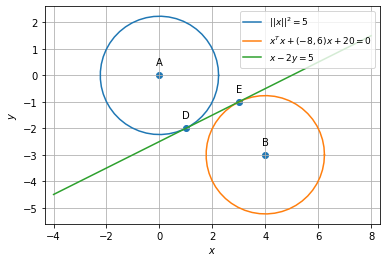
\includegraphics[width=53mm]{a_3.png}
    \caption{Graphical illustration}
    \label{fig:my_label}
\end{figure}
\end{frame}


\begin{frame}
   \centering
    \textcolor{blue}{\Huge{\textbf{THANK YOU}}}
\end{frame}
\end{document}
